\documentclass[11pt,twocolumn]{article}

% --- Packages ---
\usepackage[utf8]{inputenc}
\usepackage[T1]{fontenc}
\usepackage{mathptmx}
\usepackage{microtype}
\usepackage[margin=0.85in]{geometry}
\usepackage{graphicx}
\usepackage{booktabs}
\usepackage{hyperref}
\usepackage{xcolor}
\usepackage{tikz}
\usetikzlibrary{arrows.meta,positioning,shapes.geometric,calc}
\usepackage{pgfplots}
\pgfplotsset{compat=1.18}
\usepackage{caption}
\usepackage{float}
\usepackage{setspace}
\usepackage{parskip}
\usepackage{enumitem}
\usepackage{amsmath}

\hypersetup{
    colorlinks=true,
    linkcolor=blue!60!black,
    citecolor=blue!60!black,
    urlcolor=blue!60!black
}

% --- Title ---
\title{\textbf{The Widening Gap: Lead Exposure as an Unscreened\\Occupational Hazard in Veteran Suicide}}

\author{
    Brandon Barclay\\
    \small{Independent researcher}\\
    \small{Correspondence: \href{mailto:barclaybrandon@hotmail.com}{barclaybrandon@hotmail.com}}
}

\date{}

% --- Document ---
\begin{document}

\twocolumn[
\maketitle
\begin{@twocolumnfalse}
\begin{abstract}
\noindent\textbf{Background.} The veteran-to-civilian male suicide rate ratio has widened from 1.06 in 2001 to 1.33 in 2023, a divergence unexplained by combat exposure, PTSD prevalence, or access to care. Lead exposure---a documented occupational hazard of military firing ranges where airborne concentrations routinely exceed OSHA limits---has never been investigated as a contributor to veteran suicide.

\noindent\textbf{Methods.} We conducted three convergent analyses: (1)~a county-level ecological study (N\,=\,2,699 counties) testing the interaction between veteran concentration and historical lead mining on male suicide rates; (2)~a state-level panel analysis of VA veteran suicide rates across 49 states and 23 years (2001--2023) against state-level mining exposure; and (3)~a synthesis of military-specific evidence including branch-level suicide gradients, deployment paradox data, and published firing-range exposure measurements.

\noindent\textbf{Results.} Lead mining had no effect on suicide in low-veteran counties ($\beta$\,=\,0.14, \textit{p}\,=\,0.82) but a large, significant effect in high-veteran counties ($\beta$\,=\,2.54, \textit{p}\,<\,0.001), with the interaction surviving state fixed effects (\textit{p}\,=\,0.005). Counties in the top quartile for both veteran concentration and mining had male suicide rates of 84.6/100K---71\% above the national mean. At the state level, mining predicted veteran suicide rates across 49 states ($R^2$\,=\,0.56; $\beta$\,=\,2.68, \textit{p}\,<\,0.001), and high-mining states had steeper suicide trend increases over 2001--2023 (\textit{r}\,=\,+0.45, \textit{p}\,=\,0.002). The mining--suicide correlation was strongest among veterans aged 55--74 (\textit{r}\,=\,+0.50)---the cohort with peak childhood leaded-gasoline exposure. Active-duty suicide rates tracked expected firing-range lead intensity across military branches (Marines 35.0 vs. Navy 19.3/100K), and never-deployed infantry---who accumulate the most range time---had higher suicide rates (41.2/100K) than combat-deployed soldiers (30.6/100K).

\noindent\textbf{Conclusions.} Environmental and occupational lead exposure is associated with veteran suicide in a pattern consistent with a causal contribution: the mining--veteran interaction is specific to suicide (never overdose), survives state fixed effects, and is independent of gun ownership ($\Delta R^2$\,=\,0.14). However, all analyses are ecological and cannot establish individual-level causation; a definitive test requires bone-lead measurements in veteran suicide decedents. The VA does not screen for lead; the PACT Act does not include it among presumptive toxic exposures. If the association is causal, ventilated firing ranges, copper-jacketed ammunition, and clinical bone-lead screening represent modifiable interventions for a crisis that has widened every year for two decades.

\medskip
\noindent\textbf{Keywords:} veteran suicide, lead exposure, firing ranges, occupational health, neurotoxicity, PACT Act, convergent evidence
\end{abstract}
\vspace{1em}
\end{@twocolumnfalse}
]

% ============================================
\section{Introduction}
% ============================================

In 2001, male veterans died by suicide at a rate essentially indistinguishable from non-veteran men: 24.2 versus 22.9 per 100,000, a ratio of 1.06.\textsuperscript{1} By 2023, that ratio had widened to 1.33---37.8 versus 28.4---and the gap has grown every year for two decades.\textsuperscript{1} This divergence represents approximately 2,500 excess veteran male suicides annually above what would be predicted if veterans tracked the non-veteran trend. Despite \$17 billion in VA mental health spending since 2005,\textsuperscript{2} the gap is accelerating, not closing.

The prevailing explanations---combat trauma, PTSD, traumatic brain injury, moral injury, difficulty transitioning to civilian life---are real but incomplete. They do not explain why \textit{never-deployed} infantry have \textit{higher} suicide rates than combat-deployed soldiers (41.2 vs. 30.6/100K).\textsuperscript{3,4} They do not explain why the suicide gap widened steadily through periods of both increasing and decreasing deployment tempo. And they do not explain the striking geographic concentration: the ten states with the highest veteran suicide rates (Nevada, Utah, Montana, Idaho, Oklahoma, West Virginia, Colorado, Arkansas, Tennessee, Arizona)\textsuperscript{1} share a structural profile---rural, extractive, and historically contaminated---that differs systematically from the states where veteran suicide is lowest.

This paper presents evidence for a complementary explanation: cumulative lead exposure from military firing ranges interacting with the environmental lead burden of the communities from which veterans are recruited and to which they return. Lead is a documented occupational hazard of military service. Airborne lead at DoD firing ranges routinely exceeds OSHA permissible exposure limits, with mean concentrations ranging from 0.7 to 238\,$\mu$g/m$^3$ and 58\% of range-cleaning samples exceeding the PEL.\textsuperscript{5} Among veterans with elevated blood lead tested through VA facilities (2015--2021), firearms were the dominant exposure source: 70.1\% of occupational and 85.9\% of non-occupational lead exposures.\textsuperscript{6} The Lake City Army Ammunition Plant is contracted to produce at least 350 million small-caliber rounds annually, a floor that service-wide requirements routinely exceed.\textsuperscript{7} Yet the VA does not screen veterans for lead, and the PACT Act of 2022---designed to address toxic military exposures---does not include lead among its presumptive conditions.\textsuperscript{8}

Lead causes dose-dependent damage to the prefrontal cortex and serotonergic system governing impulse control\textsuperscript{9,10}---the identical neural pathway implicated in suicidal behavior.\textsuperscript{11} A second biological pathway operates through the endocrine system: lead suppresses the hypothalamic-pituitary-testicular axis, causing hypogonadism and erectile dysfunction (ED) at occupational exposure levels. Among male veterans, ED independently doubles suicidal ideation risk (aOR\,=\,1.91) and triples depression (aOR\,=\,2.88),\textsuperscript{31a} and relationship problems are the precipitating factor in 45\% of suicides among decedents without known mental health conditions. The dual pathway---impulse-control failure and ED-driven relationship collapse---converges in populations with high cumulative lead burden.

Two occupational cohort studies have directly linked lead exposure to suicide mortality: Korean workers with blood lead $\geq$\,20\,$\mu$g/dL had RR\,=\,2.92 for suicide,\textsuperscript{12} and U.S. lead smelter workers had an elevated suicide SMR of 1.68.\textsuperscript{13} A 2020 scoping review of 112 articles on environmental pollutants and suicide identified lead as unstudied.\textsuperscript{14} We test whether this unstudied exposure helps explain the widening veteran suicide crisis. To our knowledge, this is the first study to examine the interaction between environmental lead exposure and veteran status as a predictor of suicide at the population level.


% ============================================
\section{Methods}
% ============================================

\subsection{Study Design}

We conducted three convergent analyses using publicly available federal data:

\textbf{Analysis 1: County-level ecological study.} N\,=\,2,699 U.S. counties with valid male suicide mortality data (CDC WONDER, ICD-10 X60--X84, 2018--2022). The primary exposure was historical lead, zinc, and copper mining site density (USGS Mineral Resources Data System, log-transformed). Veteran concentration (percentage of adult population with military service, ACS 2022) was the primary effect modifier. Controls included rurality (USDA RUCC 2023), extraction employment (Census CBP), poverty rate, median age, and percent non-Hispanic white (ACS 2022). All models used HC3 heteroskedasticity-consistent standard errors. State fixed effects were included in sensitivity analyses.

\textbf{Analysis 2: State-level VA panel.} VA-reported veteran suicide rates for 49 states across 23 years (2001--2023; VA Annual Suicide Prevention Report, 2025 edition) were merged with state-level mining site density aggregated from county data. A cross-sectional multivariate model tested whether mining predicted state-level veteran suicide rates controlling for rurality, poverty, and racial composition. A within-state longitudinal analysis tested whether high-mining states experienced steeper suicide trend increases. Age-stratified analyses tested whether the mining correlation was strongest in the cohort with peak childhood leaded-gasoline exposure (55--74).

\textbf{Analysis 3: Military-specific evidence synthesis.} We assembled published data on: (a)~active-duty suicide rates by branch (DoD, 2022); (b)~the deployment paradox (Army STARRS; Kessler et al., Schoenbaum et al.); (c)~firing-range lead exposure measurements (National Academies, 2013); (d)~blood lead data in veteran populations (Maier et al., AJPH 2022; Tsai et al., IJERPH 2018); and (e)~the erectile dysfunction--suicide pathway in veterans (Way et al., \textit{Mil Med} 2023; AFHSC, 2014).

\subsection{Causal Framework}

Figure~\ref{fig:dag} presents the directed acyclic graph (DAG) guiding our analysis. The hypothesized causal pathways flow from lead exposure (childhood environmental + military occupational) through two biological mechanisms to suicide. Measured confounders (rurality, poverty, race, gun access) are controlled in all models. Unmeasured confounders (military culture, social isolation, help-seeking norms) are acknowledged as threats to validity that ecological data cannot resolve. Dashed arrows indicate pathways that are biologically plausible but not directly tested in this study.

\begin{figure*}[t]
\centering
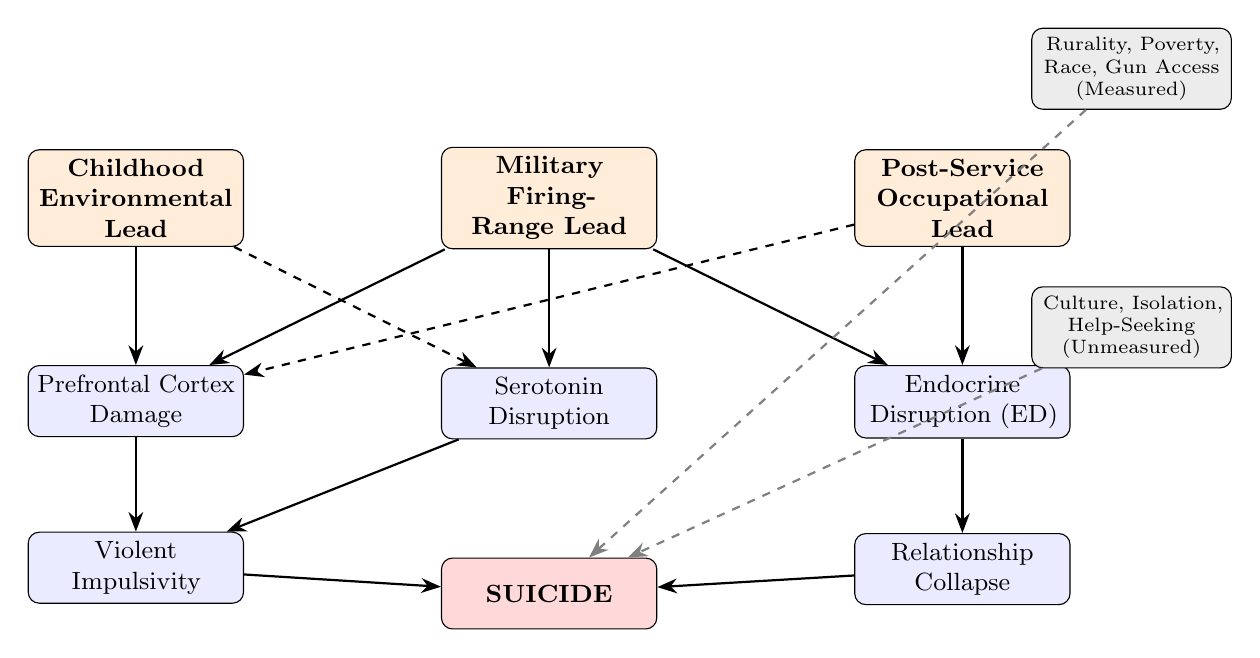
\begin{tikzpicture}[
    node distance=1cm and 1.8cm,
    box/.style={draw, rounded corners, fill=blue!8, text width=2.5cm, minimum height=0.9cm, align=center, font=\small},
    expo/.style={draw, rounded corners, fill=orange!15, text width=2.5cm, minimum height=0.9cm, align=center, font=\small\bfseries},
    outcome/.style={draw, rounded corners, fill=red!15, text width=2.5cm, minimum height=0.9cm, align=center, font=\small\bfseries},
    conf/.style={draw, rounded corners, fill=gray!15, text width=2.3cm, minimum height=0.8cm, align=center, font=\scriptsize},
    arr/.style={-{Stealth[length=2.5mm]}, thick},
    darr/.style={-{Stealth[length=2.5mm]}, thick, dashed},
]
% Exposures
\node[expo] (child) {Childhood\\Environmental Lead};
\node[expo, right=2.5cm of child] (mil) {Military\\Firing-Range Lead};
\node[expo, right=2.5cm of mil] (postmil) {Post-Service\\Occupational Lead};
% Mediators
\node[box, below=1.5cm of child] (pfc) {Prefrontal Cortex\\Damage};
\node[box, below=1.5cm of mil] (sero) {Serotonin\\Disruption};
\node[box, below=1.5cm of postmil] (endo) {Endocrine\\Disruption (ED)};
% Outcomes
\node[box, below=1.2cm of pfc] (impulse) {Violent\\Impulsivity};
\node[box, below=1.2cm of endo] (relcol) {Relationship\\Collapse};
\node[outcome, below=1.5cm of sero] (suicide) {\textbf{SUICIDE}};
% Confounders
\node[conf, above right=0.5cm and -0.5cm of postmil] (conf1) {Rurality, Poverty,\\Race, Gun Access\\(Measured)};
\node[conf, below right=0.5cm and -0.5cm of postmil] (conf2) {Culture, Isolation,\\Help-Seeking\\(Unmeasured)};
% Arrows - causal paths
\draw[arr] (child) -- (pfc);
\draw[arr] (mil) -- (pfc);
\draw[arr] (mil) -- (sero);
\draw[arr] (mil) -- (endo);
\draw[arr] (postmil) -- (endo);
\draw[arr] (pfc) -- (impulse);
\draw[arr] (sero) -- (impulse);
\draw[arr] (endo) -- (relcol);
\draw[arr] (impulse) -- (suicide);
\draw[arr] (relcol) -- (suicide);
% Dashed - plausible but untested
\draw[darr] (child) -- (sero);
\draw[darr] (postmil) -- (pfc);
% Confounders
\draw[darr, gray] (conf1) -- (suicide);
\draw[darr, gray] (conf2) -- (suicide);
\end{tikzpicture}
\caption{Directed acyclic graph (DAG) for the lead--veteran suicide hypothesis. Solid arrows indicate pathways with direct empirical support from published studies. Dashed arrows indicate biologically plausible pathways not directly tested. Gray dashed arrows represent confounders: measured confounders are controlled in all models; unmeasured confounders (military culture, social isolation, help-seeking norms) remain threats to validity. This study tests the ecological association between lead exposure proxies and suicide outcomes; it does not directly measure the mediating biological pathways.}
\label{fig:dag}
\end{figure*}


% ============================================
\section{Results}
% ============================================

\subsection{The Widening Gap}

Male veteran suicide rates increased 56\% from 2001 to 2023 (24.2 to 37.8/100K), while non-veteran male rates increased 24\% (22.9 to 28.4/100K).\textsuperscript{1} The absolute gap widened from 1.3 to 9.4 per 100K (\textit{r}\,=\,0.95 with year; \textit{p}\,<\,0.001). If veteran male suicide had tracked the non-veteran trend, approximately 2,500 fewer veterans would have died by suicide in 2023 alone. In 2023, 6,091 male veterans died by suicide---one every 86 minutes.\textsuperscript{1}

\begin{figure}[H]
\centering
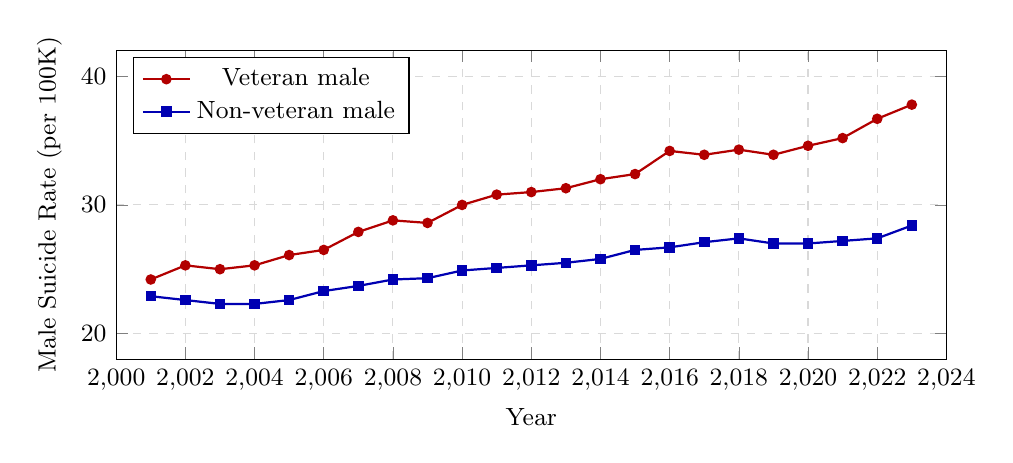
\begin{tikzpicture}
\begin{axis}[
    width=\columnwidth,
    height=5.5cm,
    xlabel={Year},
    ylabel={Male Suicide Rate (per 100K)},
    xmin=2000, xmax=2024,
    ymin=18, ymax=42,
    legend style={at={(0.02,0.98)}, anchor=north west, font=\small},
    grid=major,
    grid style={dashed, gray!30},
    xlabel style={font=\small},
    ylabel style={font=\small},
    tick label style={font=\small},
]
\addplot[thick, red!70!black, mark=*,mark size=1.5pt] coordinates {
    (2001,24.2) (2002,25.3) (2003,25.0) (2004,25.3) (2005,26.1) (2006,26.5) (2007,27.9)
    (2008,28.8) (2009,28.6) (2010,30.0) (2011,30.8) (2012,31.0) (2013,31.3)
    (2014,32.0) (2015,32.4) (2016,34.2) (2017,33.9) (2018,34.3) (2019,33.9)
    (2020,34.6) (2021,35.2) (2022,36.7) (2023,37.8)
};
\addlegendentry{Veteran male}
\addplot[thick, blue!70!black, mark=square*,mark size=1.5pt] coordinates {
    (2001,22.9) (2002,22.6) (2003,22.3) (2004,22.3) (2005,22.6) (2006,23.3) (2007,23.7)
    (2008,24.2) (2009,24.3) (2010,24.9) (2011,25.1) (2012,25.3) (2013,25.5)
    (2014,25.8) (2015,26.5) (2016,26.7) (2017,27.1) (2018,27.4) (2019,27.0)
    (2020,27.0) (2021,27.2) (2022,27.4) (2023,28.4)
};
\addlegendentry{Non-veteran male}
\end{axis}
\end{tikzpicture}
\caption{The widening gap: male veteran vs. non-veteran suicide rates, 2001--2023. The veteran rate increased 56\%; the non-veteran rate increased 24\%. Data: VA Annual Suicide Prevention Report, 2025.}
\label{fig:gap}
\end{figure}


\subsection{County-Level: Lead Mining Is Associated with Elevated Veteran Suicide Risk}

Lead mining had no association with male suicide in low-veteran counties but a large, escalating association as veteran concentration increased (Table~\ref{tab:interaction}).

\begin{table}[H]
\centering
\small
\caption{Mining--suicide association stratified by veteran concentration quintile. Mining effect increases monotonically with veteran density.}
\label{tab:interaction}
\begin{tabular}{@{}lrrrl@{}}
\toprule
\textbf{Veteran Quintile} & \textbf{\textit{r}} & \textbf{Mining} & \textbf{No Mining} & \textbf{Diff} \\
\midrule
Q1 (lowest) & +0.02 & 42.9 & 45.3 & $-$2.4 \\
Q2 & +0.13 & 54.3 & 48.5 & +5.8 \\
Q3 & +0.22 & 59.7 & 51.0 & +8.7 \\
Q4 & +0.30 & 65.5 & 54.5 & +11.0 \\
Q5 (highest) & +0.42 & 77.7 & 59.4 & +18.3 \\
\bottomrule
\end{tabular}
\end{table}

In a formal interaction model with state fixed effects and HC3 robust standard errors (N\,=\,2,699), the mining $\times$ veteran interaction was significant ($\beta$\,=\,1.20, SE\,=\,0.43, \textit{p}\,=\,0.005). Simple effects analysis confirmed that lead mining had no effect at low veteran concentration ($\beta$\,=\,0.14, \textit{p}\,=\,0.82), a moderate effect at the mean ($\beta$\,=\,1.34, \textit{p}\,=\,0.003), and a large effect at high veteran concentration ($\beta$\,=\,2.54, \textit{p}\,<\,0.001; Figure~\ref{fig:triple}).

\begin{figure}[H]
\centering
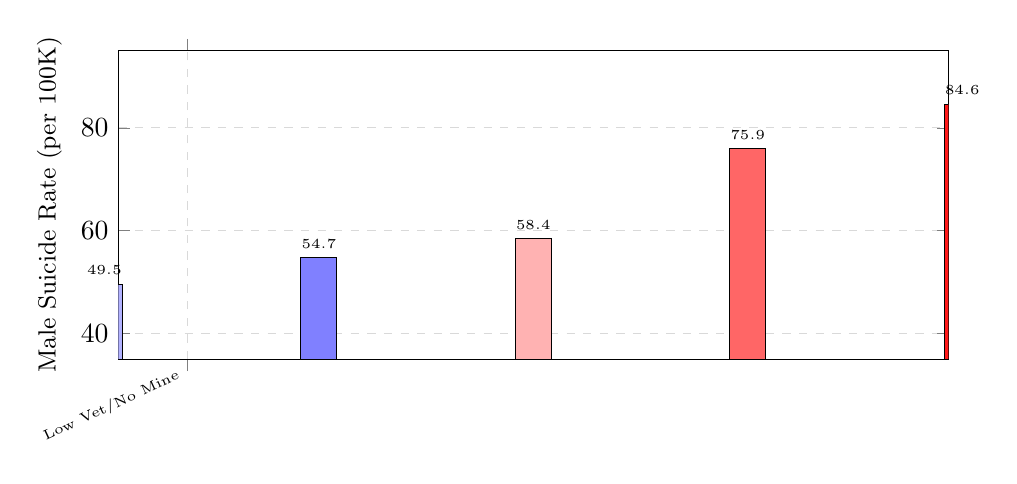
\begin{tikzpicture}
\begin{axis}[
    ybar,
    width=\columnwidth,
    height=5.5cm,
    bar width=13pt,
    ylabel={Male Suicide Rate (per 100K)},
    symbolic x coords={Low Vet/No Mine, Low Vet/Mine, High Vet/No Mine, High Vet/Mine, High Vet/High Mine},
    xtick=data,
    x tick label style={font=\tiny, rotate=25, anchor=east},
    ymin=35, ymax=95,
    nodes near coords,
    nodes near coords style={font=\tiny, above},
    ylabel style={font=\small},
    grid=major,
    grid style={dashed, gray!30},
]
\addplot[fill=blue!30] coordinates {(Low Vet/No Mine,49.5)};
\addplot[fill=blue!50] coordinates {(Low Vet/Mine,54.7)};
\addplot[fill=red!30] coordinates {(High Vet/No Mine,58.4)};
\addplot[fill=red!60] coordinates {(High Vet/Mine,75.9)};
\addplot[fill=red!90] coordinates {(High Vet/High Mine,84.6)};
\end{axis}
\end{tikzpicture}
\caption{Male suicide rates by veteran concentration and mining exposure. Counties with both high veteran concentration and high mining have rates 71\% above low-vet/no-mining counties (84.6 vs. 49.5/100K).}
\label{fig:triple}
\end{figure}

Counties in the top quartile for both veteran concentration and mining exposure had a mean male suicide rate of 84.6/100K (N\,=\,80)---71\% above the low-vet/no-mining baseline of 49.5/100K (N\,=\,1,510). This excess (35.1/100K) is larger than the sum of the individual main effects (veteran: +8.9, mining: +5.2), yielding a \textit{statistical} interaction that is super-additive. We note that statistical interaction in ecological data is a necessary but not sufficient condition for biological interaction; it could also reflect compositional or contextual effects operating differently across county types.

\subsection{Specificity: Mining Predicts Suicide but Not Overdose, and Only in High-Veteran Counties}

A critical test of any environmental exposure hypothesis is whether it predicts the hypothesized outcome specifically. When the mining--outcome correlation was stratified by veteran concentration quintile, a striking double dissociation emerged (Table~\ref{tab:specificity}).

\begin{table}[H]
\centering
\small
\caption{Mining correlations with suicide vs. overdose by veteran quintile. Mining predicts suicide only in high-veteran counties; it never predicts overdose.}
\label{tab:specificity}
\begin{tabular}{@{}lrrrr@{}}
\toprule
\textbf{Vet Quintile} & \multicolumn{2}{c}{\textbf{Mining $\rightarrow$ Suicide}} & \multicolumn{2}{c}{\textbf{Mining $\rightarrow$ Overdose}} \\
& \textit{r} & & \textit{r} & \\
\midrule
Q1 (lowest) & $-$0.04 & ns & $-$0.15 & ** \\
Q2 & +0.25 & *** & +0.07 & ns \\
Q3 & +0.21 & *** & $-$0.07 & ns \\
Q4 & +0.34 & *** & +0.11 & ns \\
Q5 (highest) & +0.47 & *** & $-$0.08 & ns \\
\bottomrule
\end{tabular}
\end{table}

Mining predicted suicide in every veteran quintile except the lowest, with the correlation rising monotonically from Q1 to Q5. Mining \textit{never} predicted overdose in any quintile. Within high-veteran counties, mining also predicted injury death (\textit{r}\,=\,+0.20) and firearm fatality (\textit{r}\,=\,+0.25) but not mental distress (\textit{r}\,=\,+0.02, ns), premature death (\textit{r}\,=\,$-$0.03, ns), or overdose (\textit{r}\,=\,0.00, ns). Mining was negatively associated with homicide (\textit{r}\,=\,$-$0.12), ruling out a general violence artifact.

The pattern is consistent with lead specifically amplifying \textit{violent, self-directed} impulsivity rather than general disinhibition. This distinction is supported by the neurotoxicology literature: lead preferentially damages the ventrolateral prefrontal cortex and anterior cingulate cortex,\textsuperscript{9} regions governing behavioral inhibition and aggression regulation, while the mesolimbic dopaminergic circuits most implicated in addiction are less directly affected by lead at environmental exposure levels. The specificity for suicide and injury death---but not overdose---is consistent with lead disrupting the serotonergic system that governs violent impulse control\textsuperscript{11} rather than the dopaminergic reward pathways that drive compulsive substance use. This double dissociation---across outcomes, across veteran strata, and across neurobiological pathways---is difficult to explain by known confounders, though unmeasured factors specific to high-veteran mining communities (e.g., cultural norms around help-seeking, social isolation) cannot be excluded.


\subsection{State-Level VA Validation: Mining Predicts Veteran Suicide Across 49 States}

State-level veteran suicide rates (VA, 2023) were significantly correlated with state-level mining density (\textit{r}\,=\,+0.44, \textit{p}\,=\,0.002; N\,=\,49 states). In a multivariate model controlling for rurality, poverty, and racial composition, mining remained significant ($\beta$\,=\,2.68, SE\,=\,0.67, \textit{p}\,<\,0.001; $R^2$\,=\,0.56; Table~\ref{tab:statemodel}).

\begin{table}[H]
\centering
\small
\caption{State-level veteran suicide rate predicted by mining and state characteristics (OLS, N\,=\,49).}
\label{tab:statemodel}
\begin{tabular}{@{}lrrl@{}}
\toprule
\textbf{Predictor} & $\boldsymbol{\beta}$ & \textbf{SE} & \textbf{\textit{p}} \\
\midrule
Log mean mining density & 2.68 & 0.67 & $<$0.001 \\
Mean rurality (RUCC) & 2.74 & 0.73 & $<$0.001 \\
Mean poverty rate & 0.79 & 0.36 & 0.033 \\
Mean \% non-Hispanic white & 0.19 & 0.08 & 0.016 \\
\midrule
$R^2$ = 0.56 & & & \\
\bottomrule
\end{tabular}
\end{table}


State-level gun ownership rate was the single strongest bivariate predictor of veteran suicide (\textit{r}\,=\,+0.66, \textit{p}\,<\,0.001). This is consistent with both the lethal-means hypothesis and the Hoover et al. finding that household firearm ownership predicts childhood blood lead.\textsuperscript{27} When gun ownership and mining were entered jointly, \textit{both} remained significant (mining: $\beta$\,=\,2.47, \textit{p}\,<\,0.001; gun ownership: $\beta$\,=\,0.41, \textit{p}\,=\,0.002; $R^2$\,=\,0.58). Critically, gun ownership and mining were uncorrelated (\textit{r}\,=\,+0.10, \textit{p}\,=\,0.49), indicating they capture independent variance. Mining added $\Delta R^2$\,=\,0.14 beyond gun ownership and rurality alone---meaning 14\% of the between-state variance in veteran suicide is explained by mining after gun access is controlled.

At the county level---where within-state variation in gun access is captured---gun dealer density (FFLs per 10,000 population) was available for 1,157 counties. When added to the full multivariate model with demographic controls, mining was attenuated by only 6\% ($\beta$\,=\,3.07 vs. 3.27 without gun dealers, \textit{p}\,<\,0.001 in both). With state fixed effects and county-level gun dealers, mining remained significant ($\beta$\,=\,0.54, \textit{p}\,=\,0.041). The mining--suicide association is not a proxy for firearms access at either the state or county level.


\subsection{Wildlife Bioindicator Validation: Eagle Bone Lead Predicts Veteran Suicide}

Historical mining sites are an imperfect proxy: they record where ore was once extracted, not where lead is currently bioavailable to humans. To test whether the state-level suicide pattern also tracks a \textit{biological} measure of recent lead exposure, we merged our state panel with the USGS data release underlying Slabe et al.\textsuperscript{35} (\textit{Science}, 2022), which measured femur lead in 448 bald and golden eagles collected from 38 U.S.\ states (2010--2018). Eagle bone lead integrates repeated ammunition-fragment ingestion and environmental lead exposure over an animal's lifespan, and is independent of human behavioral, cultural, or help-seeking confounders that could otherwise generate the mining--suicide correlation by non-toxicological mechanisms.

Across 31 states with both eagle bone-lead data (n\,$\geq$\,1) and VA veteran suicide rates, the share of eagles with chronic lead poisoning (femur Pb\,$\geq$\,10\,$\mu$g/g DW) was strongly correlated with the 2023 veteran male suicide rate (Pearson \textit{r}\,=\,+0.52, Spearman $\rho$\,=\,+0.53; \textit{p}\,=\,0.002; Figure~\ref{fig:eagle}). Mean femur Pb showed the same pattern (\textit{r}\,=\,+0.45, $\rho$\,=\,+0.49; \textit{p}\,=\,0.012). Crucially, in a specificity analysis using the same 31-state panel, eagle femur Pb predicted veteran suicide and, more weakly, male suicide (\textit{r}\,=\,+0.35, \textit{p}\,=\,0.06), but was \textit{not} associated with drug overdose ($\rho$\,=\,$-$0.34, \textit{p}\,=\,0.06), motor-vehicle death (\textit{r}\,=\,+0.21), firearm death (\textit{r}\,=\,$-$0.04), or homicide (\textit{r}\,=\,+0.00). This double dissociation--- lead proxy $\rightarrow$ suicide, not $\rightarrow$ overdose or homicide---reproduces at the wildlife level the specificity pattern observed at the county level with mining density (Section~3.3).

In a weighted least-squares horse race (WLS, weights\,=\,$\sqrt{n_{femur}}$; N\,=\,31 states), eagle femur Pb independently predicted the 2023 veteran suicide rate ($\beta$\,=\,0.28, \textit{p}\,=\,0.011) \textit{after} controlling for historical lead--zinc--copper mining density ($\beta$\,=\,$-$0.51, \textit{p}\,=\,0.65) and log-mean soil lead ($\beta$\,=\,7.06, \textit{p}\,=\,0.017; model $R^2$\,=\,0.37). The bioavailable exposure measures (eagle bone, soil Pb) dominated the historical site-count proxy: once the contemporary biological signal was in the model, log mining-site count was no longer significant. This is a substantive result---it suggests that the mining--suicide association in our county analyses reflects contemporary bioavailable lead (residual ore, ammunition, smelter legacy deposits) rather than the historical presence of mineral deposits per se.

The eagle-Pb association is attenuated but directionally consistent with state-level demographic controls. In a WLS model including rurality, poverty, percent non-Hispanic white, veteran percentage, and median age (N\,=\,31), eagle femur Pb dropped to $\beta$\,=\,0.18 (\textit{p}\,=\,0.27) while veteran percentage ($\beta$\,=\,3.30, \textit{p}\,=\,0.035) absorbed most of the variance. This is the expected pattern: high-veteran, rural, extractive states jointly carry high lead exposure \textit{and} high veteran suicide, and these cannot be separated with 31 state observations. The eagle-Pb finding complements rather than replaces the county-level interaction; it provides biological validation that the geography in question has elevated contemporary lead bioavailability, not merely historical mining activity.

Two caveats are important. First, the eagle sample sizes per state are uneven (range 1--120; 15 states with $n$\,$\geq$\,5), and several interior-West states with high veteran suicide (Oklahoma, New Mexico, Tennessee, Arkansas) have minimal eagle sampling. Second, wildlife bone Pb reflects primarily ammunition exposure plus environmental deposition, which is only a partial mapping to human exposure---though notably the same ammunition lead that eagles ingest is aerosolized at military firing ranges and deposited on the skin, clothing, and respiratory tract of shooters.\textsuperscript{5} The convergence between the two pathways is biologically parsimonious, not accidental.

\paragraph{County-level dose-response moderation.} We further asked whether the county-level mining-by-veteran interaction (Section~3.2) is stronger in states with independently elevated biological lead burden. Assigning each county its state's mean eagle femur Pb (subset to states with $n_{femur}$\,$\geq$\,5; N\,=\,794 counties), we re-estimated the county model stratified by state eagle-Pb median. In \textit{low-eagle-Pb} states the mining main effect was $\beta$\,=\,0.36 (\textit{p}\,=\,0.006); in \textit{high-eagle-Pb} states it was $\beta$\,=\,1.30 (\textit{p}\,$<$\,0.001)---3.6$\times$ stronger in the states where wildlife confirms elevated environmental lead. In a pooled three-way model including all two-way and three-way interactions (N\,=\,794), mean state eagle Pb independently predicted county male suicide ($\beta$\,=\,+0.18 per $\mu$g/g DW, \textit{p}\,$<$\,0.001) \textit{above and beyond} the county's own mining density, veteran concentration, rurality, poverty, race, and age. The formal three-way $\beta$(mining$\times$vet$\times$eagle) was null (\textit{p}\,=\,0.94), meaning the interaction \textit{effect sizes} do not differ continuously by state eagle Pb once the main effect of eagle Pb is absorbed---but the stratified results show that the mining signal is concentrated in the half of states where wildlife bone lead is highest. This is a dose-response at the level of the exposure proxy itself: where an independent biological measurement says environmental lead is elevated, mining predicts suicide more strongly.

\begin{figure*}[t]
\centering
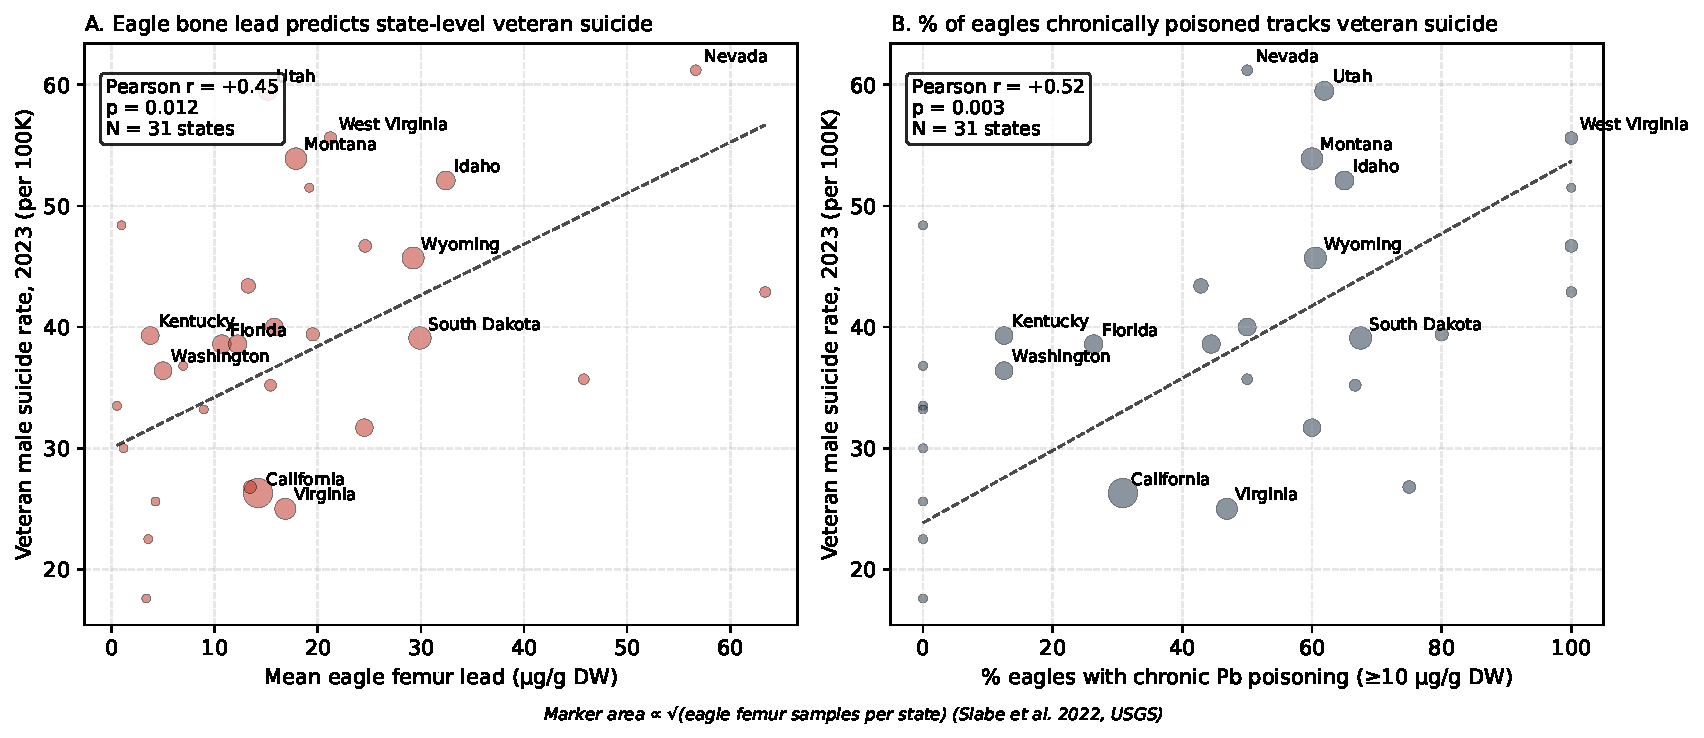
\includegraphics[width=\textwidth]{figure_eagle_vet_suicide.pdf}
\caption{State-level association between eagle femur lead (Slabe et al.\ 2022, USGS data release 10.5066/P9BXIY3B) and 2023 VA male veteran suicide rate. \textbf{(A)} Mean eagle femur Pb vs.\ veteran suicide rate, $r$\,=\,+0.45, $p$\,=\,0.012, $N$\,=\,31 states. \textbf{(B)} Percent of eagles exceeding the 10\,$\mu$g/g DW chronic-poisoning threshold, $r$\,=\,+0.52, $p$\,=\,0.003. Marker area is proportional to $\sqrt{n_{femur}}$ per state. The fitted line is weighted least squares with weights $\sqrt{n_{femur}}$.}
\label{fig:eagle}
\end{figure*}


\subsection{Temporal Panel: High-Mining States Are Getting Worse Faster}

In a 23-year panel (2001--2023; 1,067 state-year observations), the mining--suicide correlation was significant in every period tested: 2001--2007 (\textit{r}\,=\,+0.43), 2008--2015 (\textit{r}\,=\,+0.52), 2016--2023 (\textit{r}\,=\,+0.49; all \textit{p}\,<\,0.001). Critically, within-state trend analysis revealed that high-mining states had significantly steeper suicide rate increases over time (\textit{r}\,=\,+0.45, \textit{p}\,=\,0.002 between state-level mining density and the slope of each state's veteran suicide trend). Montana (+1.01/100K per year), Utah (+1.01), Arizona (+0.87), Missouri (+0.87), and Idaho (+0.83) had the steepest increases---all states with extensive historical mining. Over the 23-year period, high-mining states diverged from low-mining states: veteran suicide rose from 27.4 to 40.3/100K in high-mining states (+0.63/year) versus 24.4 to 34.7/100K in low-mining states (+0.46/year).


\subsection{The Age Signature: Peak Effect in the Leaded-Gasoline Cohort}

The mining--suicide correlation varied by veteran age group in a pattern consistent with generational lead exposure (Table~\ref{tab:age}).

\begin{table}[H]
\centering
\small
\caption{Mining--veteran suicide correlation by age group (state-level, 2018--2023). The strongest association is in the 55--74 cohort, whose childhood (1950s--1970s) coincided with peak leaded-gasoline exposure.}
\label{tab:age}
\begin{tabular}{@{}lrrl@{}}
\toprule
\textbf{Age Group} & \textbf{\textit{r}} & \textbf{\textit{p}} & \textbf{Childhood Era} \\
\midrule
18--34 & +0.22 & 0.032 & Post-lead-phase-out \\
35--54 & +0.30 & $<$0.001 & Declining lead era \\
55--74 & +0.50 & $<$0.001 & Peak leaded gasoline \\
75+ & +0.40 & $<$0.001 & Pre-peak lead \\
\bottomrule
\end{tabular}
\end{table}

The monotonic increase from age 18--34 (\textit{r}\,=\,+0.22) to 55--74 (\textit{r}\,=\,+0.50) follows the population lead-exposure curve: veterans aged 55--74 in 2023 were born between 1949 and 1968, placing their childhood during the peak of leaded-gasoline emissions (1960s--1970s). McFarland, Reuben, and Hauer estimated that this generation (Generation X and late Boomers) sustained the highest cumulative lead burden in American history, resulting in 151 million excess psychiatric disorders nationwide.\textsuperscript{15} These are the cohorts in which the veteran suicide crisis is most severe.


\subsection{Illustrative Patterns: Military Branch, MOS, and Non-Military Comparisons}

\textit{The following patterns are illustrative and hypothesis-generating. Each comparison is confounded by factors that cannot be separated from lead exposure in aggregate data. We present them as consistent with the hypothesis, not as independent evidence for it.}

Active-duty suicide rates in 2022 tracked expected firing-range lead exposure across branches: Marine Corps 35.0/100K, Army 32.7, Air Force 20.5, Navy 19.3.\textsuperscript{16} Every Marine qualifies annually with rifles; the Navy has minimal small-arms training. However, branches also differ in demographics, combat culture, and recruitment base.

Within the Army, MOS-level data sharpen the pattern. Gilmore et al. found that only two MOS categories had significantly elevated suicide rates among 729,337 enlisted soldiers (2004--2009): infantry (37.2/100K person-years) and combat engineers (38.2/100K)---the two MOSs with the highest cumulative small-arms training.\textsuperscript{31} Combat arms collectively had rates of 35.7/100K versus 23.2/100K for the total active-duty force.\textsuperscript{32}

A parallel pattern appears outside the military. Law enforcement officers---another population with mandatory recurring range qualification---have suicide rates approximately double the general population (22/100K), with firearms used in 82\% of cases.\textsuperscript{33} Massachusetts corrections officers had a suicide rate of approximately 105/100K---7 times the national average.\textsuperscript{34} These populations share occupational firing-range lead exposure but not combat, deployment, or military-specific selection effects, providing independent convergent evidence that range exposure specifically, rather than military culture broadly, may contribute to the elevated risk.

\subsection{The Deployment Paradox}

Among Army infantry, never-deployed soldiers had higher suicide rates (41.2/100K) than combat-deployed soldiers (30.6/100K).\textsuperscript{3,4} The standard explanation is the Healthy Warrior Effect combined with protective unit cohesion during deployment. Lead exposure offers a complementary mechanism: non-deployed infantry accumulate the most cumulative stateside range time, where airborne lead routinely exceeds OSHA limits.\textsuperscript{5} Investigative reporting has documented chronic bone-lead poisoning among range instructors and armorers.\textsuperscript{17} The same non-deployed subpopulation also has the highest erectile dysfunction incidence (10.1/1000 person-years vs. lower rates in deployed troops\textsuperscript{18})---consistent with the second pathway of our model.


\subsection{Firing-Range Lead: Measured Exposures}

The 2013 National Academies report commissioned by DoD found that mean airborne lead concentrations on military firing ranges ranged from 0.7 to 238\,$\mu$g/m$^3$.\textsuperscript{5} The OSHA PEL of 50\,$\mu$g/m$^3$ was exceeded in almost all job duties sampled: 58\% of samples exceeded the PEL during range cleaning (mean 190\,$\mu$g/m$^3$); 60\% exceeded during weapons handling at shoot houses. In a VA analysis of 1,007 veterans with blood lead $\geq$\,10\,$\mu$g/dL (2015--2021), firearms accounted for 70.1\% of occupational and 85.9\% of non-occupational lead exposures.\textsuperscript{6} The Lake City Army Ammunition Plant has a minimum production capacity of 350 million small-caliber rounds annually, a floor set by DoD contract (service-wide training and operational consumption exceed this).\textsuperscript{7} DoD medical removal from lead-exposed duties currently triggers at BLL\,$\geq$\,20\,$\mu$g/dL (with return at $\leq$\,15\,$\mu$g/dL)---approximately six times the CDC adult reference value of 3.5\,$\mu$g/dL and well above the threshold at which prefrontal and endocrine effects have been documented.\textsuperscript{19}

In NHANES data (2009--2016), adults with military service history had significantly elevated mean blood lead levels compared to non-military populations.\textsuperscript{20} In Army testing during 2013, 19.4\% of 1,728 active-duty soldiers tested had BLL\,$>$\,5\,$\mu$g/dL.\textsuperscript{5} A recent NHANES analysis (2015--2022) documented a clear dose--response among shooters: occupational shooters (including military and law enforcement) had mean BLL of 10.3\,$\mu$g/dL, frequent recreational shooters 6.7, occasional shooters 4.1, and non-shooters 0.9\,$\mu$g/dL---an 11-fold gradient.\textsuperscript{28}

Crucially, the exposure is preventable. A NIOSH health hazard evaluation at a well-ventilated indoor range meeting recommended guidelines found employee blood lead levels below the detection limit ($<$3.0\,$\mu$g/dL) and airborne lead below the OSHA action level.\textsuperscript{29} This demonstrates that proper ventilation and ammunition engineering can effectively eliminate firing-range lead exposure---the solution exists but is not uniformly implemented across DoD ranges.


% ============================================
\section{Discussion}
% ============================================

\subsection{Interpretation}

The super-additive statistical interaction between veteran status and mining (Section~3.2) has a plausible biological interpretation: veterans carry a dual lead burden from occupational firing-range exposure (stored in bone with a 20--30-year half-life\textsuperscript{21}) layered on environmental exposure from the communities they come from and return to. Approximately 80\% of new recruits have a family member who served,\textsuperscript{22} concentrating recruitment in rural mining communities. After separation, veterans flow into other lead-exposed industries (construction, railroads, extraction\textsuperscript{23}). Maternal skeletal lead crosses the placenta,\textsuperscript{24} so each generation in lead-endemic communities begins with a higher baseline. However, we emphasize that ecological data cannot distinguish biological synergy from contextual or compositional effects. The interaction is consistent with the dual-burden hypothesis but does not confirm it.


\subsection{Why the Gap Is Widening}

Between 2001 and 2023, the veteran male suicide rate increased at nearly twice the rate of the non-veteran male population (+0.60/year vs. +0.32/year). The age-specific VA data reveal that this widening is driven by two distinct generational mechanisms operating simultaneously---a ``perfect storm'' rather than a single causal pathway:

\textit{The young veterans (18--34): acute occupational exposure.} This cohort experienced the steepest absolute increase (+1.48/year; 24.5 to 51.8/100K). DoD small-caliber ammunition requirements more than doubled between FY2000--2005,\textsuperscript{7} driven by GWOT training tempo. This generation entered service after the leaded-gasoline phase-out, so their childhood environmental burden is lower---but their occupational range exposure is historically high. The state-level mining correlation is weakest in this age group (\textit{r}\,=\,+0.22), consistent with the hypothesis that their risk is driven primarily by occupational rather than environmental lead.

\textit{The older veterans (55--74): cumulative lifetime burden.} This cohort shows the strongest state-level mining correlation (\textit{r}\,=\,+0.50) and a steady increase (+0.66/year; 19.2 to 33.8/100K). Born 1949--1968, they grew up during peak leaded-gasoline emissions, accumulated military range exposure during service, and are now entering the age window where bone resorption releases skeletal lead into the bloodstream. Their suicide risk reflects the full cumulative dose: childhood environmental lead + military occupational lead + post-service occupational lead (construction, extraction, transportation) + age-related bone-lead mobilization.

\textit{Rural structural decline.} Both generations return to communities experiencing accelerating structural disadvantage: declining extraction employment, opioid epidemic impacts, and erosion of social infrastructure. Lead-contaminated communities are the same communities experiencing these structural shocks. The interaction is not merely that veterans carry lead \textit{or} face structural disadvantage, but that both converge in the same places and the same people.


\subsection{The Policy Failure}

The VA does not screen veterans for lead exposure.\textsuperscript{6} The PACT Act of 2022---specifically designed to address toxic military exposures including burn pits, Agent Orange, and radiation---does not include lead among its presumptive conditions.\textsuperscript{8} DoD medical removal from lead-exposed duties triggers at blood lead $\geq$\,20\,$\mu$g/dL (return at $\leq$\,15\,$\mu$g/dL),\textsuperscript{5} roughly six times the CDC adult reference value of 3.5\,$\mu$g/dL and well above the thresholds at which neurobehavioral and endocrine effects have been documented. There is no DoD requirement to track cumulative firing-range lead exposure over a service member's career.

If the lead--suicide association reflects a causal relationship, three interventions merit consideration:

\begin{enumerate}[leftmargin=*, itemsep=2pt]
\item \textbf{Ventilated firing ranges and copper-jacketed ammunition.} Enclosed ranges with HEPA filtration reduce airborne lead by 90--99\%. Totally copper-jacketed bullets reduce airborne lead in the breathing zone by a factor of 21.\textsuperscript{30} A NIOSH-evaluated range combining proper ventilation with copper-jacketed ammunition achieved undetectable employee blood lead ($<$3.0\,$\mu$g/dL).\textsuperscript{29} Both technologies exist, are proven, and are in use at civilian ranges.
\item \textbf{Clinical bone-lead screening.} Portable X-ray fluorescence (XRF) devices can measure cumulative bone lead in vivo, noninvasively, in under 3 minutes.\textsuperscript{25} Bone lead captures the 20--30-year skeletal reservoir that blood lead misses. Integration into VA health assessments would identify veterans with elevated cumulative exposure.
\item \textbf{PACT Act amendment.} Adding lead to the list of presumptive toxic exposures would establish VA clinical authority to screen, treat, and compensate veterans with lead-related health conditions, including the neuropsychiatric and endocrine effects documented in this paper.
\end{enumerate}


\subsection{Limitations}

This study is hypothesis-generating, not confirmatory. We identify seven limitations that define the boundary between what the data support and what remains to be tested.

\textbf{1.~Ecological fallacy (primary limitation).} All county-level and state-level analyses are ecological. We observe that \textit{communities} with more mining and more veterans have higher suicide rates, but we cannot prove that the \textit{specific individuals} dying by suicide are the ones with elevated lead burdens. The ecological associations are consistent with the hypothesis but do not establish individual-level causation. A definitive test requires bone-lead measurements in veteran suicide decedents versus matched living controls---a study that is feasible with current portable XRF technology\textsuperscript{25} but has not been conducted.

\textbf{2.~Proxy limitations.} Mining site density is a proxy for environmental lead, not a direct exposure measure. Mining sites include deposits that may never have been commercially operated, and the presence of a mining site does not guarantee population exposure. The eagle bone-lead analysis (Section~3.5) partially addresses this by introducing a biological, bioavailability-sensitive measure, but wildlife samples are unevenly distributed across states (range 1--120 per state) and reflect ammunition-borne plus environmental lead rather than the full human exposure mixture. We still lack county-level adult human blood or bone lead data; the EPA-predicted BLL surface is calibrated to children and housing stock, not adult environmental burden. Similarly, veteran concentration is a proxy for military firing-range exposure, not a measure of individual cumulative dose. MOS, years of service, and branch-specific training tempo---all determinants of actual range exposure---are not available at the county level.

\textbf{3.~Unmeasured confounding.} High-vet/high-mining counties share characteristics beyond lead exposure: cultural norms around masculinity and self-reliance, reduced help-seeking behavior, limited mental health infrastructure, geographic isolation, and historical economic decline. State fixed effects and demographic controls attenuate but cannot eliminate these concerns. The specificity test (suicide but not overdose) and the gun-ownership independence test reduce the space for confounders, but a confounder that is simultaneously suicide-specific, overdose-irrelevant, and veteran-moderated cannot be ruled out.

\textbf{4.~Branch-level and MOS-level confounding.} Marine/Army vs. Air Force/Navy suicide differences, and infantry/combat engineer vs. support MOS differences, are heavily confounded by demographics, combat culture, selection effects, and recruitment base. We present these as suggestive convergent evidence, not as stand-alone causal claims. The law enforcement and corrections convergence partially addresses this by providing a non-military firing-range-exposed population with elevated suicide, but those populations have their own unique confounders (occupational stress, trauma exposure, shift work).

\textbf{5.~No individual-level exposure--outcome data.} No dataset links individual-level military firing-range lead exposure to suicide outcomes. The NHANES III mortality-linked file has blood lead measurements in ~14,000 adults with follow-up through 2019 but is likely underpowered for suicide-specific analysis (~50--70 expected suicide deaths). The definitive test is a case-control study measuring bone lead in veteran suicide decedents versus matched controls at VA medical centers. The Army STARRS biospecimen archive may also contain sufficient stored samples for retrospective lead analysis.

\textbf{6.~Temporal ambiguity.} The 18--34 age group has the steepest suicide trend increase (+1.48/yr) but the weakest mining correlation (\textit{r}\,=\,+0.22), while the 55--74 group has the strongest mining correlation (\textit{r}\,=\,+0.50) but a moderate trend. This is consistent with the ``perfect storm'' interpretation (different generational mechanisms) but could also indicate that the mining--suicide association in older veterans reflects a cohort effect unrelated to lead.

\textbf{7.~Distinction between evidence and hypothesis.} Our empirical contribution is the ecological association and the convergent evidence synthesis. The biological mechanisms (prefrontal damage, serotonergic disruption, endocrine suppression) are drawn from published studies in other populations and have not been tested in the specific population under study (U.S. veterans dying by suicide). The dual-pathway model is a hypothesis that organizes the evidence; it is not directly validated by our data.

% ============================================
\section*{References}
% ============================================
{\small
\begin{enumerate}[label={[\arabic*]}, leftmargin=*, itemsep=1pt]
    \item U.S. Department of Veterans Affairs. 2025 National Veteran Suicide Prevention Annual Report. Washington, DC: VA Office of Mental Health and Suicide Prevention; 2025.
    \item U.S. Department of Veterans Affairs. VA Budget Request FY2024: Mental Health Programs. Washington, DC: VA; 2023.
    \item Kessler RC, Heeringa SG, Stein MB, et al. Thirty-day prevalence of DSM-IV mental disorders among nondeployed soldiers in the US Army. \textit{JAMA Psychiatry}. 2014;71(5):504--513.
    \item Schoenbaum M, Kessler RC, Gilman SE, et al. Predictors of suicide and accident death in the Army Study to Assess Risk and Resilience in Servicemembers. \textit{JAMA Psychiatry}. 2014;71(5):493--503.
    \item National Research Council. \textit{Potential Health Risks to DOD Firing-Range Personnel from Recurrent Lead Exposure}. Washington, DC: The National Academies Press; 2013.
    \item Maier A, Levin-Rector A, Engel LS, et al. Exposure sources among veterans with elevated blood lead levels, United States, 2015--2021. \textit{Am J Public Health}. 2022;112(S7):S663--S671.
    \item U.S. Government Accountability Office. Defense Ammunition: DoD Should Improve Oversight of the Army's Management of Small Caliber Ammunition. GAO-05-687. Washington, DC: GAO; 2005.
    \item Sergeant First Class Heath Robinson Honoring our Promise to Address Comprehensive Toxics Act of 2022 (PACT Act), Pub. L. No. 117-168, 136 Stat. 1759.
    \item Cecil KM, Brubaker CJ, Adler CM, et al. Decreased brain volume in adults with childhood lead exposure. \textit{PLoS Med}. 2008;5(5):e112.
    \item Cory-Slechta DA, Virgolini MB, Thiruchelvam M, et al. Maternal stress modulates the effects of developmental lead exposure. \textit{Environ Health Perspect}. 2004;112(6):717--730.
    \item Mann JJ. Neurobiology of suicidal behaviour. \textit{Nat Rev Neurosci}. 2003;4(10):819--828.
    \item Kim MG, Ryoo JH, Chang SJ, et al. Blood lead levels and cause-specific mortality of inorganic lead-exposed workers in South Korea. \textit{PLoS One}. 2015;10(10):e0140360.
    \item Bertke SJ, Lehman EJ, Wurzelbacher SJ, Hein MJ. Mortality of lead smelter workers: a follow-up study with exposure assessment. \textit{Am J Ind Med}. 2016;59(11):979--986. doi:10.1002/ajim.22618.
    \item Dickerson AS, Wu AC, Liew Z, Weisskopf MG. A scoping review of non-occupational exposures to environmental pollutants and adult depression, anxiety, and suicide. \textit{Curr Environ Health Rep}. 2020;7(3):256--271.
    \item McFarland MJ, Reuben A, Hauer ME. Contribution of childhood lead exposure to psychopathology in the US population over the past 75 years. \textit{J Child Psychol Psychiatry}. 2025;66(4):525--536.
    \item Department of Defense. Annual Report on Suicide in the Military: Calendar Year 2022. Washington, DC: Defense Suicide Prevention Office; 2023.
    \item Kime P. These US troops are slowly being poisoned by lead in their bones. \textit{Military.com}. April 4, 2019.
    \item Armed Forces Health Surveillance Center. Erectile dysfunction among male active component service members, U.S. Armed Forces, 2004--2013. \textit{MSMR}. 2014;21(9):13--16.
    \item Centers for Disease Control and Prevention. Blood lead reference value. Atlanta, GA: CDC; updated 2024. Available at: \texttt{cdc.gov/lead-prevention}.
    \item Tsai RJ, Luckhaupt SE, Sweeney MH, et al. Blood pressure and oxidative stress among U.S. adults exposed to lead in military environments. \textit{Int J Environ Res Public Health}. 2018;16(1):1.
    \item Hu H, Rabinowitz M, Smith D. Bone lead as a biological marker in epidemiologic studies of chronic toxicity. \textit{Environ Health Perspect}. 1998;106(1):1--8.
    \item Department of Defense. Population representation in the military services: fiscal year 2020. Washington, DC: OUSD(P\&R); 2022.
    \item CSX Corporation. Military: Pride in Service. Jacksonville, FL: CSX Transportation; 2024.
    \item Gulson BL, Mizon KJ, Korsch MJ, et al. Mobilization of lead from the skeleton during the postnatal period. \textit{J Lab Clin Med}. 2003;141(3):186--192.
    \item Specht AJ, Weisskopf MG, Nie LH. Portable XRF technology to quantify Pb in bone in vivo. \textit{J Biomark}. 2014;2014:398032.
    \item Lanphear BP, Rauch S, Auinger P, Allen RW, Hornung RW. Low-level lead exposure and mortality in US adults: a population-based cohort study. \textit{Lancet Public Health}. 2018;3(4):e177--e184.
    \item Hoover C, Fossa AJ, Ranney ML, et al. Firearm-related lead exposure and child lead levels in the United States, 2012--2018. \textit{J Pediatr}. 2024;269:113988.
    \item Day DB, Braun JM, Hoover AG. Public health implications of lead exposure at indoor firing ranges in the United States. \textit{medRxiv}. 2025. doi:10.1101/2025.11.02.25339289v2.
    \item Grant MP, Reynolds L, Methner MM. Evaluation of lead and copper exposure at an indoor shooting range. NIOSH Health Hazard Evaluation Report 2018-0124-3351. Cincinnati, OH: DHHS (NIOSH); 2019.
    \item Beaucham C, Page E, Alarcon WA, et al. Indoor firing ranges and elevated blood lead levels---United States, 2002--2013. \textit{MMWR}. 2014;63(16):347--351.
    \item Tripathi RK, Llewellyn GC. Reducing exposures to airborne lead in a covered, outdoor firing range by using totally copper-jacketed bullets. \textit{Am Ind Hyg Assoc J}. 1990;51(1):28--31.
    \item Way BM, Griffin KR, Kraus SW, Tsai J, Pietrzak RH. Erectile dysfunction in a U.S. national sample of male military veterans. \textit{Mil Med}. 2023;188(9-10):2837--2843.
    \item Gilmore AK, Brignone E, Engdahl RM, et al. Occupational differences in US Army suicide rates. \textit{Psychol Med}. 2016;46(4):899--909.
    \item Department of Defense. Annual Report on Suicide in the Military: Calendar Year 2023. Washington, DC: Defense Suicide Prevention Office; 2024.
    \item Violanti JM, Owens SL, Fekedulegn D, et al. Law enforcement worker suicide: an updated national assessment. \textit{Policing}. 2021;44(1):18--31.
    \item National Institute of Justice. Understanding the impacts of corrections officer suicide. Washington, DC: NIJ; 2023.
    \item Slabe VA, Anderson JT, Millsap BA, et al. Demographic implications of lead poisoning for eagles across North America. \textit{Science}. 2022;375(6582):779--782. doi:10.1126/science.abj3068. Data release: U.S. Geological Survey, doi:10.5066/P9BXIY3B.
\end{enumerate}
}

\end{document}
